\documentclass[12pt,a4paper]{report}
\usepackage{indentfirst}

\usepackage[margin=1in]{geometry}
\usepackage{graphicx}
\usepackage{array}
\usepackage{booktabs}
\usepackage{float}
\usepackage{setspace}
\usepackage{titlesec}
\usepackage{tocloft}
\usepackage{enumitem}
\usepackage{hyperref}
\usepackage{xcolor}
\usepackage{url}
\usepackage{eso-pic}
\usepackage{tikz}
\usepackage{fancyhdr}
\usepackage{lastpage}
\usepackage{etoolbox}

\hypersetup{
    colorlinks=true,
    linkcolor=black,
    urlcolor=blue,
    pdftitle={Internship Report},
    pdfauthor={Kamal S}
}

% -- Spacing ----------------------------------------------------------------
\setstretch{1.15}
%\setlength{\parindent}{1.5em}
\setlength{\parskip}{0.4em}

% -- Chapter heading format -------------------------------------------------
\titleformat{\chapter}[display]
  {\filcenter\bfseries\Large}
  {\chaptername~\thechapter}{10pt}{\LARGE}

\titlespacing*{\chapter}
{0pt}
{-10pt}
{35pt}

% Ensure chapter marks are set for headers
\renewcommand{\chaptermark}[1]{\markboth{#1}{#1}}

% -- Rename TOC / LOF headings to match template ----------------------------
\renewcommand{\contentsname}{TABLE OF CONTENTS}
\renewcommand{\listfigurename}{LIST OF FIGURES}

% -- TOC heading format (consistent with other front-matter headings) -------
\renewcommand{\cfttoctitlefont}{\hfill\LARGE\bfseries}
\renewcommand{\cftaftertoctitle}{\hfill}
\renewcommand{\cftloftitlefont}{\hfill\LARGE\bfseries}
\renewcommand{\cftafterloftitle}{\hfill}
\setlength{\cftbeforetoctitleskip}{-1.5em}
\setlength{\cftaftertoctitleskip}{1.5em}
\setlength{\cftbeforeloftitleskip}{-1.5em}
\setlength{\cftafterloftitleskip}{1.5em}
\renewcommand{\cftsecleader}{\cftdotfill{\cftdotsep}}
\renewcommand{\cftchapleader}{\cftdotfill{\cftdotsep}}

% -- Toggle: border ON/OFF --------------------------------------------------
% We define a boolean that controls whether borders are drawn.
% Front-matter pages: border ON.  Chapter pages: border OFF.
\newif\ifshowborder
\showbordertrue  % start with borders ON

\AddToShipoutPictureBG{%
  \ifshowborder
  \begin{tikzpicture}[remember picture, overlay]
    \draw[line width=0.56pt]
      ([xshift=18pt, yshift=-18pt]current page.north west)
      rectangle
      ([xshift=-18pt, yshift=18pt]current page.south east);
    \draw[line width=0.28pt]
      ([xshift=20pt, yshift=-20pt]current page.north west)
      rectangle
      ([xshift=-20pt, yshift=20pt]current page.south east);
  \end{tikzpicture}%
  \fi
}

% -- Page styles ------------------------------------------------------------

% Style for front-matter: no header/footer, just centered page number
\fancypagestyle{frontmatter}{
  \fancyhf{}
  \renewcommand{\headrulewidth}{0pt}
  \renewcommand{\footrulewidth}{0pt}
  \fancyfoot[C]{\thepage}
}

% Style for main content: header + footer, no border
\fancypagestyle{mainchapter}{
  \fancyhf{}
  \renewcommand{\headrulewidth}{0.4pt}
  \renewcommand{\footrulewidth}{0.4pt}
  \fancyhead[L]{\small FullStack developer}
  \fancyhead[R]{\small\nouppercase{\leftmark}}
  \fancyfoot[L]{\small Dept. of ECE, Vemana IT}
  \fancyfoot[C]{\small 2025-2026}
  \fancyfoot[R]{\small Page \thepage\ of \pageref{LastPage}}
  \renewcommand{\chaptermark}[1]{\markboth{##1}{}}
}

% Plain style for front-matter (used by \chapter*, \listoffigures, etc.)
% Initially just centered page number. Redefined before main content.
\fancypagestyle{plain}{
  \fancyhf{}
  \renewcommand{\headrulewidth}{0pt}
  \renewcommand{\footrulewidth}{0pt}
  \fancyfoot[C]{\thepage}
}

\begin{document}
\setlength{\parindent}{0pt}
% ==========================================================================
% TITLE PAGE  (single-spaced, zero parskip so it fits on one page)
% ==========================================================================
\begin{titlepage}
\thispagestyle{empty}
\begin{singlespacing}
\setlength{\parskip}{0pt}
%\setlength{\parindent}{0pt}
\centering
\vspace*{-0.5cm}

{\Large \textbf{VISVESVARAYA TECHNOLOGICAL UNIVERSITY}\par}
\vspace{2pt}
{\large \textbf{Jnana Sangama, Belagavi -- 590018}\par}
\vspace{8pt}

\includegraphics[height=5cm]{images/vtu_logo.png}\par
\vspace{8pt}
{\itshape An Internship Report\par}
\vspace{2pt}
{\itshape On\par}
\vspace{4pt}
{\LARGE \textbf{\textquotedblleft FullStack developer\textquotedblright}\par}
\vspace{4pt}
{\textcolor{red}{Jan 27 to May 2}\par}
\vspace{8pt}
{\itshape Submitted in partial fulfillment of the requirements for the award of the degree of\par}
\vspace{4pt}
{\large \textbf{Bachelor of Engineering}\par}
\vspace{2pt}
{\large \textbf{in}\par}
\vspace{2pt}
{\large \textbf{\textcolor{black}{Electronics and communication Engineering}}\par}
\vspace{8pt}
Submitted by\par
\vspace{4pt}
{\large \textbf{KAMAL S \hspace{2cm} 1VI22EC066}\par}
\vspace{10pt}

\includegraphics[height=4cm]{images/vit_logo.png}\par
\vspace{10pt}
{\large \textbf{DEPARTMENT OF ELECTRONICS AND COMMUNICATION ENGINEERING}\par}
{\Large \textbf{VEMANA INSTITUTE OF TECHNOLOGY}\par}
{\large BENGALURU -- 560034\par}
\vspace{6pt}
{\Large \textbf{2025-2026}\par}

\end{singlespacing}
\end{titlepage}

% ==========================================================================
% FRONT MATTER — borders ON, roman numbering, no headers/footers
% ==========================================================================
\pagenumbering{roman}
\pagestyle{frontmatter}

% ==========================================================================
% CERTIFICATE PAGE
% ==========================================================================

\thispagestyle{empty}

% Watermark
\AddToShipoutPictureFG*{%
\begin{tikzpicture}[remember picture,overlay]
\node[opacity=0.05] at ([yshift=-4.8cm]current page.center)
{

\includegraphics[height=7cm]{images/vit_logo.png}
};
\end{tikzpicture}
}

\begin{center}

\vspace*{-1.4cm}

{\large \textbf{Karnataka ReddyJana Sangha}}

{\Large \textbf{VEMANA INSTITUTE OF TECHNOLOGY}}\\[2pt]

{\small (Affiliated to Visvesvaraya Technological University, Belagavi)}\\[-1pt]

{\small Koramangala, Bengaluru--560034}\\[10pt]


\includegraphics[height=2.8cm]{images/dept_seal.png}\\[8pt]

{\large \textbf{DEPARTMENT OF}}\\[2pt]

{\large \textbf{ELECTRONICS AND COMMUNICATION ENGINEERING}}\\[10pt]

{\LARGE \textbf{CERTIFICATE}}

\end{center}

\vspace{0.2cm}

\noindent
This is to certify that the internship entitled \textbf{“FullStack developer”} is a bonafide work carried out by \textbf{KAMAL S (1VI22EC066)} in partial fulfillment of the requirements for the award of Bachelor of Engineering degree in \textbf{Electronics and communication Engineering}, Visvesvaraya Technological University, Belagavi, during the academic year 2025-2026.

\vspace{0.25cm}

\noindent
It is certified that all corrections and suggestions indicated for internal assessment have been duly incorporated in the report. The internship report has been approved as it satisfies the academic requirements prescribed for the said degree.

\vspace{1.2cm}

\begin{center}

\renewcommand{\arraystretch}{1.15}

\begin{tabular}{c c c c}

\textbf{Internal Supervisor} &
\textbf{External Supervisor} &
\textbf{HOD} &
\textbf{Principal}
\\[4pt]

(Prof. Suma B V) &
(Maneesh Kumar Varma) &
(Dr. Suneeta) &
(Dr. Vijayasimha Reddy B G)

\end{tabular}

\end{center}

\vspace{1cm}

\noindent
\textbf{Name of the Examiners}
\hfill
\textbf{Signature with Date}

\vspace{0.4cm}

\noindent
1.\hspace{0.2cm}\rule{5cm}{0.4pt}
\hfill
\rule{4cm}{0.4pt}

\vspace{0.4cm}

\noindent
2.\hspace{0.2cm}\rule{5cm}{0.4pt}
\hfill
\rule{4cm}{0.4pt}


% ==========================================================================
% ACKNOWLEDGEMENT
% ==========================================================================
\newpage
\setcounter{page}{2}  % Ack = page ii (certificate was empty)
\begin{center}
{\LARGE \textbf{ACKNOWLEDGEMENT}\par}
\end{center}
\addcontentsline{toc}{chapter}{Acknowledgement}

\vspace{0.5cm}
\setlength{\parskip}{1em}
\begin{onehalfspacing}
I sincerely thank Visvesvaraya Technological University (VTU) for providing me with the opportunity to undertake this internship as a part of the academic curriculum, which has contributed significantly to my learning and overall development.

I express my sincere gratitude to 	extbf{Dr. Vijayasimha Reddy B G}, Principal, Vemana Institute of Technology, Bengaluru, for providing the necessary infrastructure, encouragement, and support to successfully carry out the internship work.

I extend my heartfelt thanks to 	extbf{Dr. Suneeta}, Head of the Department, Electronics and communication Engineering, Vemana Institute of Technology, for their constant guidance, motivation, and encouragement throughout the internship duration.

I would also like to thank Internal Supervisor 	extbf{Prof. Suma B V}, External Supervisor 	extbf{Maneesh Kumar Varma}, and all Internship Coordinators for their cooperation, coordination, and support during the internship period.

I am thankful to all the teaching and non-teaching staff members of the Department of Electronics and communication Engineering for their support and encouragement throughout the internship.

I also acknowledge the support of 	extbf{Supram Technologies} for providing structured learning resources and an environment that encouraged systematic understanding, practical application, and continuous improvement.
\end{onehalfspacing}
\setlength{\parskip}{0.4em}

\vspace{1cm}
\begin{flushright}
\textbf{Kamal S}\par
1VI22EC066\par
\end{flushright}

% ==========================================================================
% ABSTRACT
% ==========================================================================
\newpage
\begin{center}
{\LARGE \textbf{ABSTRACT}\par}
\end{center}
\addcontentsline{toc}{chapter}{Abstract}

\vspace{0.5cm}
%\setlength{\parindent}{1.5em}

Abstract not provided.


% ==========================================================================
% TABLE OF CONTENTS — Standard LaTeX TOC with dotted leaders
% ==========================================================================
\newpage
\tableofcontents

% ==========================================================================
% LIST OF FIGURES — Custom table format matching template
% ==========================================================================
\newpage
% We need the custom header for LOF
\addtocontents{lof}{\textbf{Figure No} \hfill \textbf{Title} \hfill \textbf{Page No}\par\smallskip\hrule\par\bigskip}
\listoffigures

% ==========================================================================
% MAIN CONTENT — borders OFF, headers/footers ON, arabic numbering
% ==========================================================================
\newpage
\showborderfalse       % TURN OFF borders for all remaining pages
\pagenumbering{arabic}

% Redefine plain style for chapter first pages — SAME as mainchapter
% Template shows header + footer on ALL chapter pages including the first page
\fancypagestyle{plain}{
  \fancyhf{}
  \renewcommand{\headrulewidth}{0.4pt}
  \renewcommand{\footrulewidth}{0.4pt}
  \fancyhead[L]{\small FullStack developer}
  \fancyhead[R]{\small\nouppercase{\leftmark}}
  \fancyfoot[L]{\small Dept. of ECE, Vemana IT}
  \fancyfoot[C]{\small 2025-2026}
  \fancyfoot[R]{\small Page \thepage\ of \pageref{LastPage}}
  \renewcommand{\chaptermark}[1]{\markboth{##1}{}}
}
\pagestyle{mainchapter}

% ==========================================================================
% CHAPTER 1: INTRODUCTION
% ==========================================================================
\chapter{INTRODUCTION}
\label{ch:intro}



\section{Internship Scope and Objectives}


\section{Relevance of FullStack developer to Electronics and communication Engineering}


\section{Evolution of Practices in the Field}


\section{Current Trends and Technologies}




% ==========================================================================
% CHAPTER 2: ORGANISATION PROFILE
% ==========================================================================
\chapter{ORGANISATION PROFILE}
\label{ch:org}



\section{Introduction}



\begin{figure}[H]
\centering

\includegraphics[width=0.55\textwidth,height=5cm,keepaspectratio]{images/company_logo_0552f78b.png}
\caption{Internship Provider - Supram Technologies Logo}
\end{figure}


\section{Vision and Mission of the Organization}


\section{Programs and Services Offered}


\section{Organizational Impact and Reach}


\section{Core Values}




% ==========================================================================
% CHAPTER 3: WORK DONE / METHODOLOGY
% ==========================================================================
\chapter{WORK DONE / METHODOLOGY}
\label{ch:work}



\section{Overview of Internship Work}


\section{Tools and Technologies Used}




\section{Work Process and Methodology}


\section{Key Project and Case Study}



\begin{figure}[H]
\centering
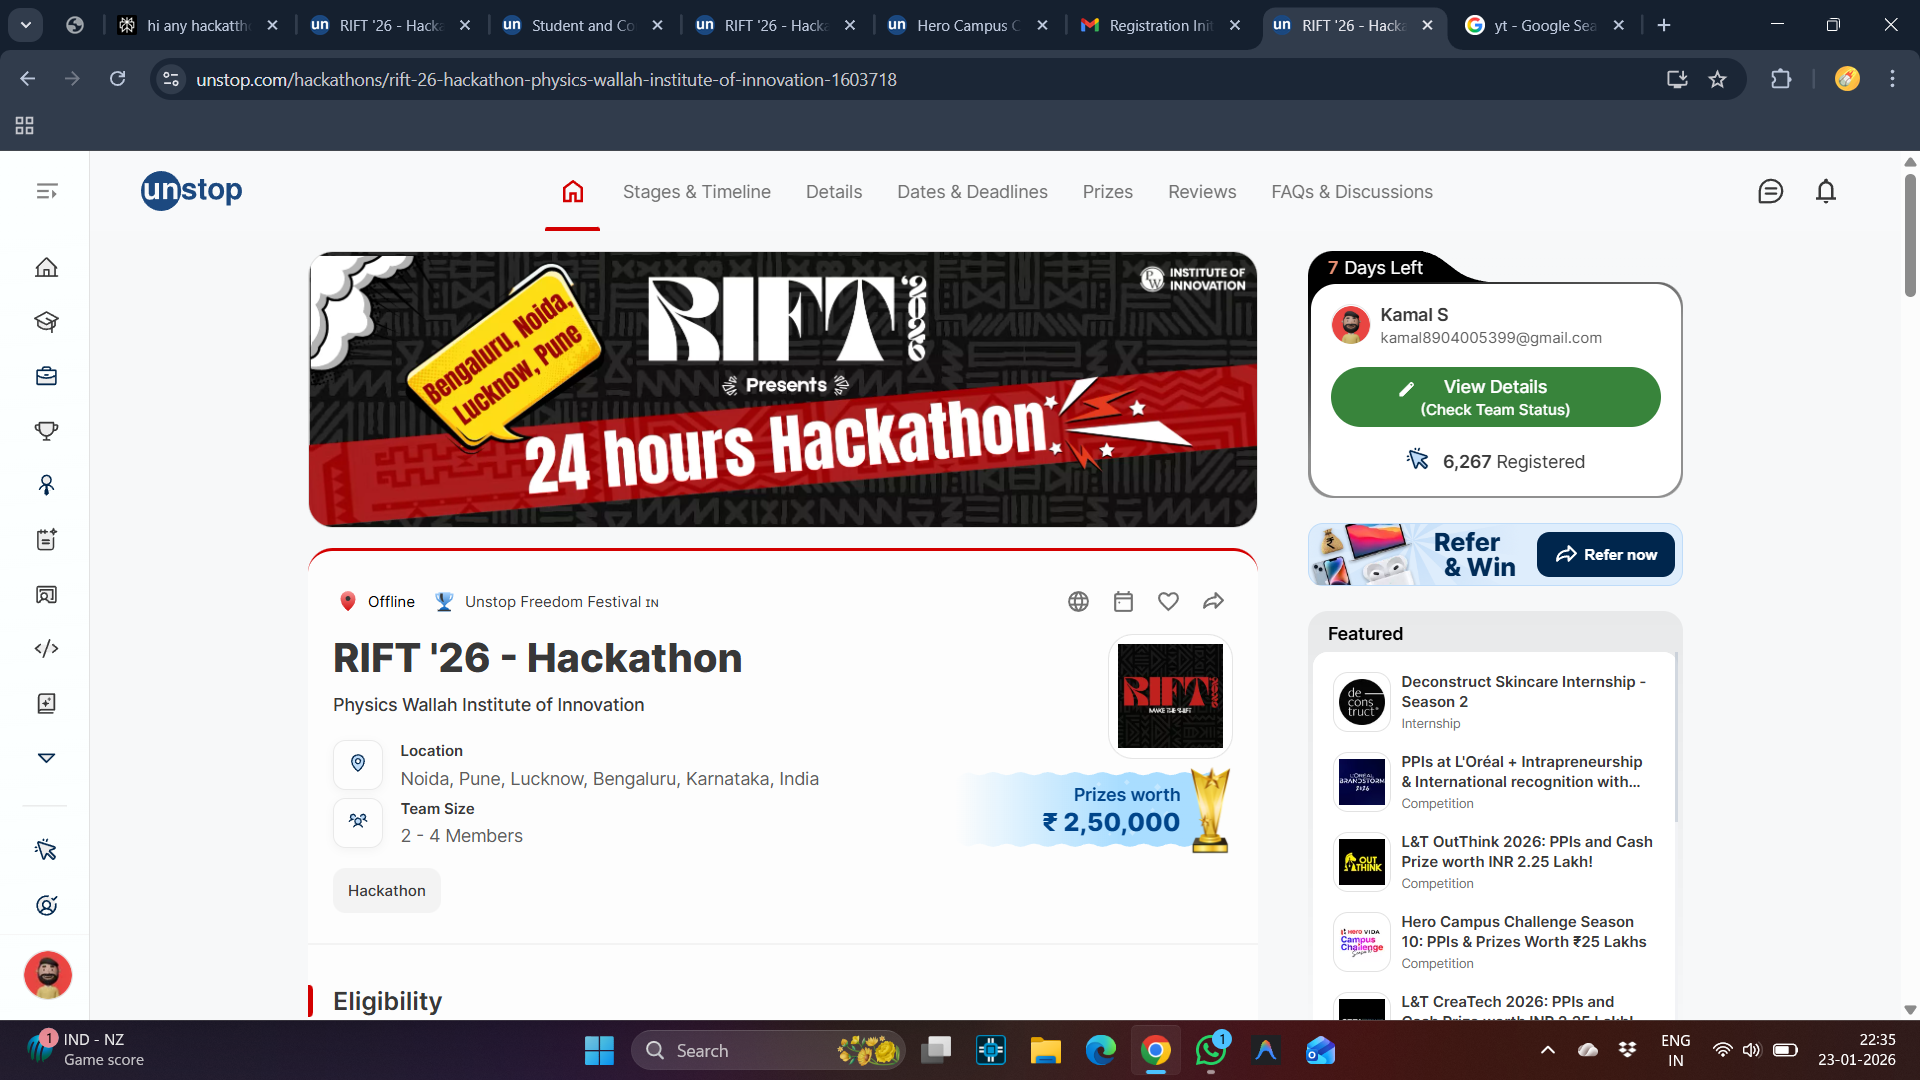
\includegraphics[width=0.45\textwidth,height=5cm,keepaspectratio]{images/ch_img_1a0bab4c.png}
\caption{Image}
\end{figure}


\section{Challenges Faced}


\section{Solutions Implemented}


% ==========================================================================
% CHAPTER 4: RESULTS AND DISCUSSION
% ==========================================================================
\chapter{RESULTS AND DISCUSSION}
\label{ch:results}





\section{Outcomes of the Work}


\section{Learning Outcomes}


\section{Analysis}




% ==========================================================================
% CHAPTER 5: CONCLUSION
% ==========================================================================
\chapter{CONCLUSION}
\label{ch:conclusion}


This chapter summarizes the overall internship experience, highlighting key outcomes, personal growth, and future directions.




\section{Summary}


\section{Personal Growth}


\section{Future Scope}


\end{document}
